\chapter{Grundlagen}
Dieses Kapitel erläutert die Grundlagen die zum 
Verständnis dieser Arbeit notwendig sind. 
Angefangen mit der Erklärung für Technologien
Docker und Kubernetes, hinzu Microservices.

%TEXT!!!!

\section{Docker} \label{Docker}

In diesem Abschnitt wird die Technologie \glqq Docker\grqq{} näher erläutert und
nicht das Unternehmen \glqq Docker, Inc.\grqq{}, dass für die maßgebliche Entwicklung dessen verantwortlich ist.
Angefangen mit der Terminologie, zum deutlicheren Verständnis der nächsten Abschnitte.
Fortgesetzt mit der aufsteigenden Erklärung der Architektur bis zum Aufbau eines Containers.

%\subsection{Terminologie}
%\begin{itemize}
%    \item \textbf{Container}: Isolierter Prozess mit einer laufenden Anwendung.
%    \item \textbf{Volumes}: Persistente Daten eines Containers.
%    \item \textbf{Image}: Einheit mit ausführbaren Code, Abhängigkeiten und Betriebssystem. Aufgeteilt in mehreren Schichten.
%    \item \textbf{Dockerfile}: Textdatei zum erstellen eines Docker-Images.    
%\end{itemize}

\subsection{Architektur}
Die Docker Technologie ist in der Programmiersprache \glqq GO\grqq{} geschrieben und nutzt Funktionalitäten des
Linux Kernels, wie cgroups und namespaces.
Namespaces ermöglichen die Isolation von Prozessen in sogenannte Container, welche unabhängig voneinander arbeiten \cite{dockergetstarted}.
Diese beeinhalten alle nötigen Abhängigkeiten zur Ausführung der vordefinierten Anwendung.
Container gewinnen dadurch an Portabilität, die ein bereitstellen auf Infrastrukturen mit der Docker
Laufzeit ermöglichen.
Die Laufzeit setzt sich aus \glqq runc\grqq{} einer low-Level Laufzeit und \glqq containerd\grqq{} einer higher-Level
Laufzeit zusammen (vgl. Abbildung~\ref{fig:dockerarch}).
Runc dient als Schnittstelle zum Betriebssystem und startet und stoppt Container.
Containerd verwaltet die Lebenszyklen eines Container, ziehen von Images, erstellen von Netzwerken und
Verwaltung von runc.
Die Allgemeine Aufgabe des Docker Daemons ist es eine vereinfachte Schnittstelle für die Abstraktion
der unterliegenden Schicht zu gewährleisten, wie zum Beispiel dem verwalten von Images, Volumes und Netzwerken \cite{dockerdeep}.
Auf die Orchestrierung mit Swarm wird nicht weiter eingeganen, da sie zum Verständnis nicht nötig ist.

\begin{figure}
    \centering
    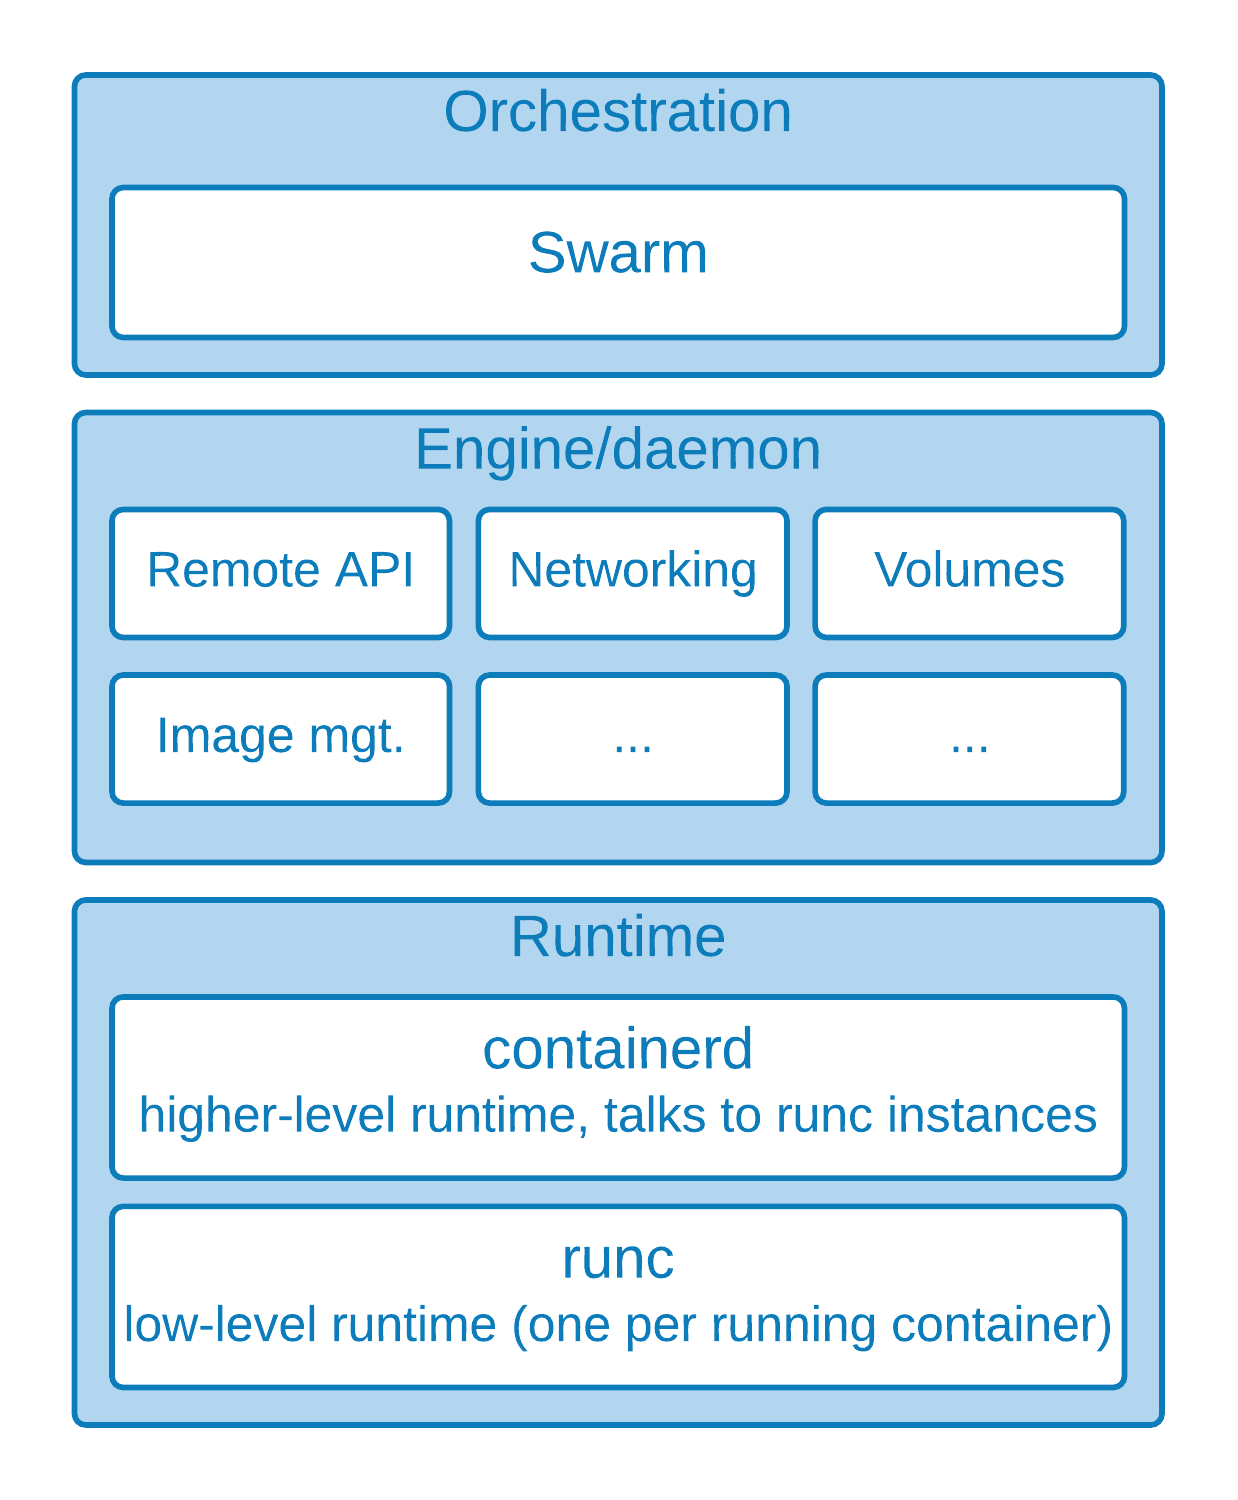
\includegraphics[width=0.5\columnwidth]{images/DockerArch.png}
    \caption{Docker Architektur \protect\cite{dockerdeep}}
    \label{fig:dockerarch}
\end{figure}

\subsection{Images und Container}
Ein Docker Image ist ein Objekt das alle Abhängigkeiten wie Quellcode, Bibliotheken und Betriebssystem
Funktionen für eine Anwendung beeinhaltet. 

\subsubsection{Registries}
Das beziehen von Images erfolgt über sogenannte \glqq Image Registries\grqq{}.
Bei Docker ist dies standardmäßig \url{https://hub.docker.com} und das eigene Lokale Registry. 
Es ist auch möglich eigene zu hosten oder die von Drittanbieter zu nutzen.

\subsubsection{Schichten}
Docker Images bestehen aus mehreren Schichten, jede davon abhängig von der Schicht unter ihr und
erkennbar durch IDs in Form von SHA256 Hashes (vgl. Abbildung~\ref{fig:dockerlayer}).
Docker kann dadurch beim bauen oder updaten von neuen Images vorhandene Schichten erneut verwenden. 
Die feste Reihenfolge ermöglicht eine ressourceneffiziente Verwaltung von Builds,
indem man oft wechselnde Schichten oben platziert. 
Die Leistung beim erstellen und zusammenführen von Schichtem hängt vom Dateisystem des Hostsystems ab.
Eine Schicht kann aus mehreren Dateien bestehen
und einzelne Dateien aus der Unterliegenden Schicht mit einer neuen ersetzen.

\begin{figure}
    \centering
    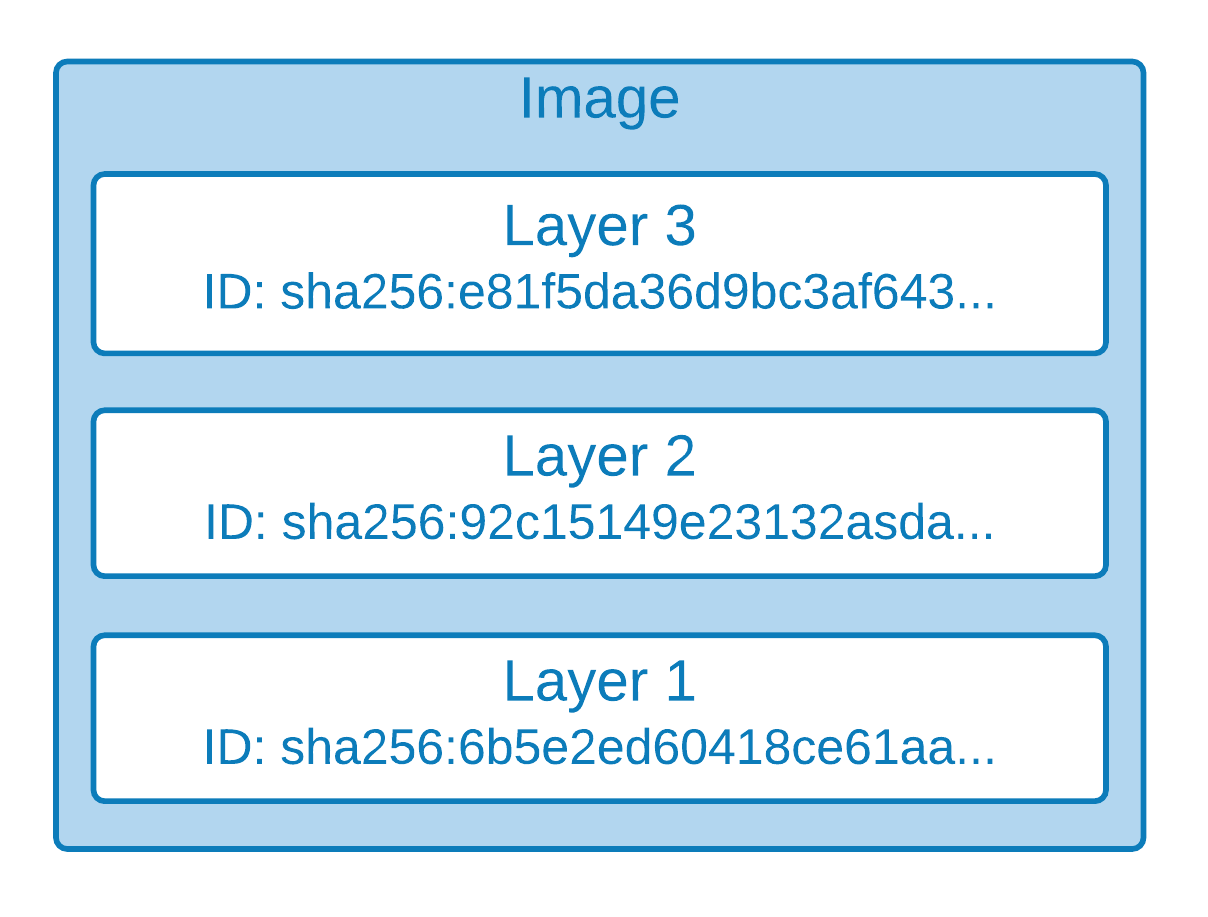
\includegraphics[width=0.5\columnwidth]{images/Image-Layer.png}
    \caption{Image Layers \protect}
    \label{fig:dockerlayer}
\end{figure}

%copy-on-write (CoW) strategy???

%nicht alle dockerfile anweisungen erstellen layer ENV expose usw.
Das starten eines Containers fügt auf die bereits bestehenden Schichten einen \glqq Thin R/W layer\grqq{} 
oder auch \glqq Container layer\grqq{} genannt hinzu, dieser gewährt Schreib- und Leserechte bei Laufzeit des Prozesses. 
Jeder dieser Container hat somit einen individuellen Zustand, der unähnlich vom abstammendem Image ist.
Bei Löschung des Containers verschwindet auch die dazu gewonne Schicht.
Das entfernen eines Images ist durch die Konzeption des Schichtensystem erst möglich, wenn alle darauf
basierenden Container gelöscht sind \cite{dockerstoragedriver}.

\subsubsection{Dockerfile}
Zur Erstellung eines Docker Images wird ein Dockerfile benötigt, dies beeinhaltet alle Anweisungen
zum Aufbau der einzelnen Schichten. 
Diese Aufrufe erstellen die Schichten eines Images \cite{dockerbestpracticedockerfile}.
\begin{itemize}
    \item \textbf{FROM} erstellen einer Schicht von einem base-image. 
    \item \textbf{COPY} hinzufügen von Dateien aus dem derzeitigen Verzeichnis. 
    \item \textbf{RUN} bauen der Anwendung mit make. 
\end{itemize}
Diese hingegen fügen nur Metadaten hinzu \cite{dockerbestpracticedockerfile}.
\begin{itemize}
    \item \textbf{EXPOSE} informiert Docker an welchem Port der Container innerhalb seines Netzwerks lauscht.
    \item \textbf{ENTRYPOINT} ermöglicht es einen Container als ausführbare Datei zu starten.
    \item \textbf{CMD} Befehl beim ausführen des Containers.
\end{itemize}


\subsection{Containervirtualisierung}
Aus dem Wissen des letzten Abschnitts lässt sich Schlussfolgern, dass
ein Container eine laufende Instanz eines Images ist.
Vergleichbar ist dieses Konzept mit dem einer virtuellen Maschine (VM).
Denn Images ermöglichen ähnlich wie VM templates, die Erstellung von mehreren Instanzen durch eine Vorkonfiguration.
Mit dem großen Unterschied, dass die Einrichtung von VMs müheseliger ist und weitaus mehr Ressourcen
beansprucht, da sie ein ganzes Betriebssystem ausführt \cite{hypervisorcontainer}. Containertechnologien bauen hingegen nur auf 
bestimmte Funktionalitäten des Kernels auf und sparen damit an Rechenleistung (vgl. Abbildung~\ref{fig:containervm}).

Durch die Vorteile eines geteilten Kernels und dessen Betriebssystem abhängigkeiten,
erzielen Virtualisierungen basierend auf Container eine höhere Anzahl an 
virtuellen Instanzen. Images sind auch um einiges kleiner als hypervisor-basierende
Ansätze \cite{hypervisorcontainer}.

\begin{figure}
    \centering
    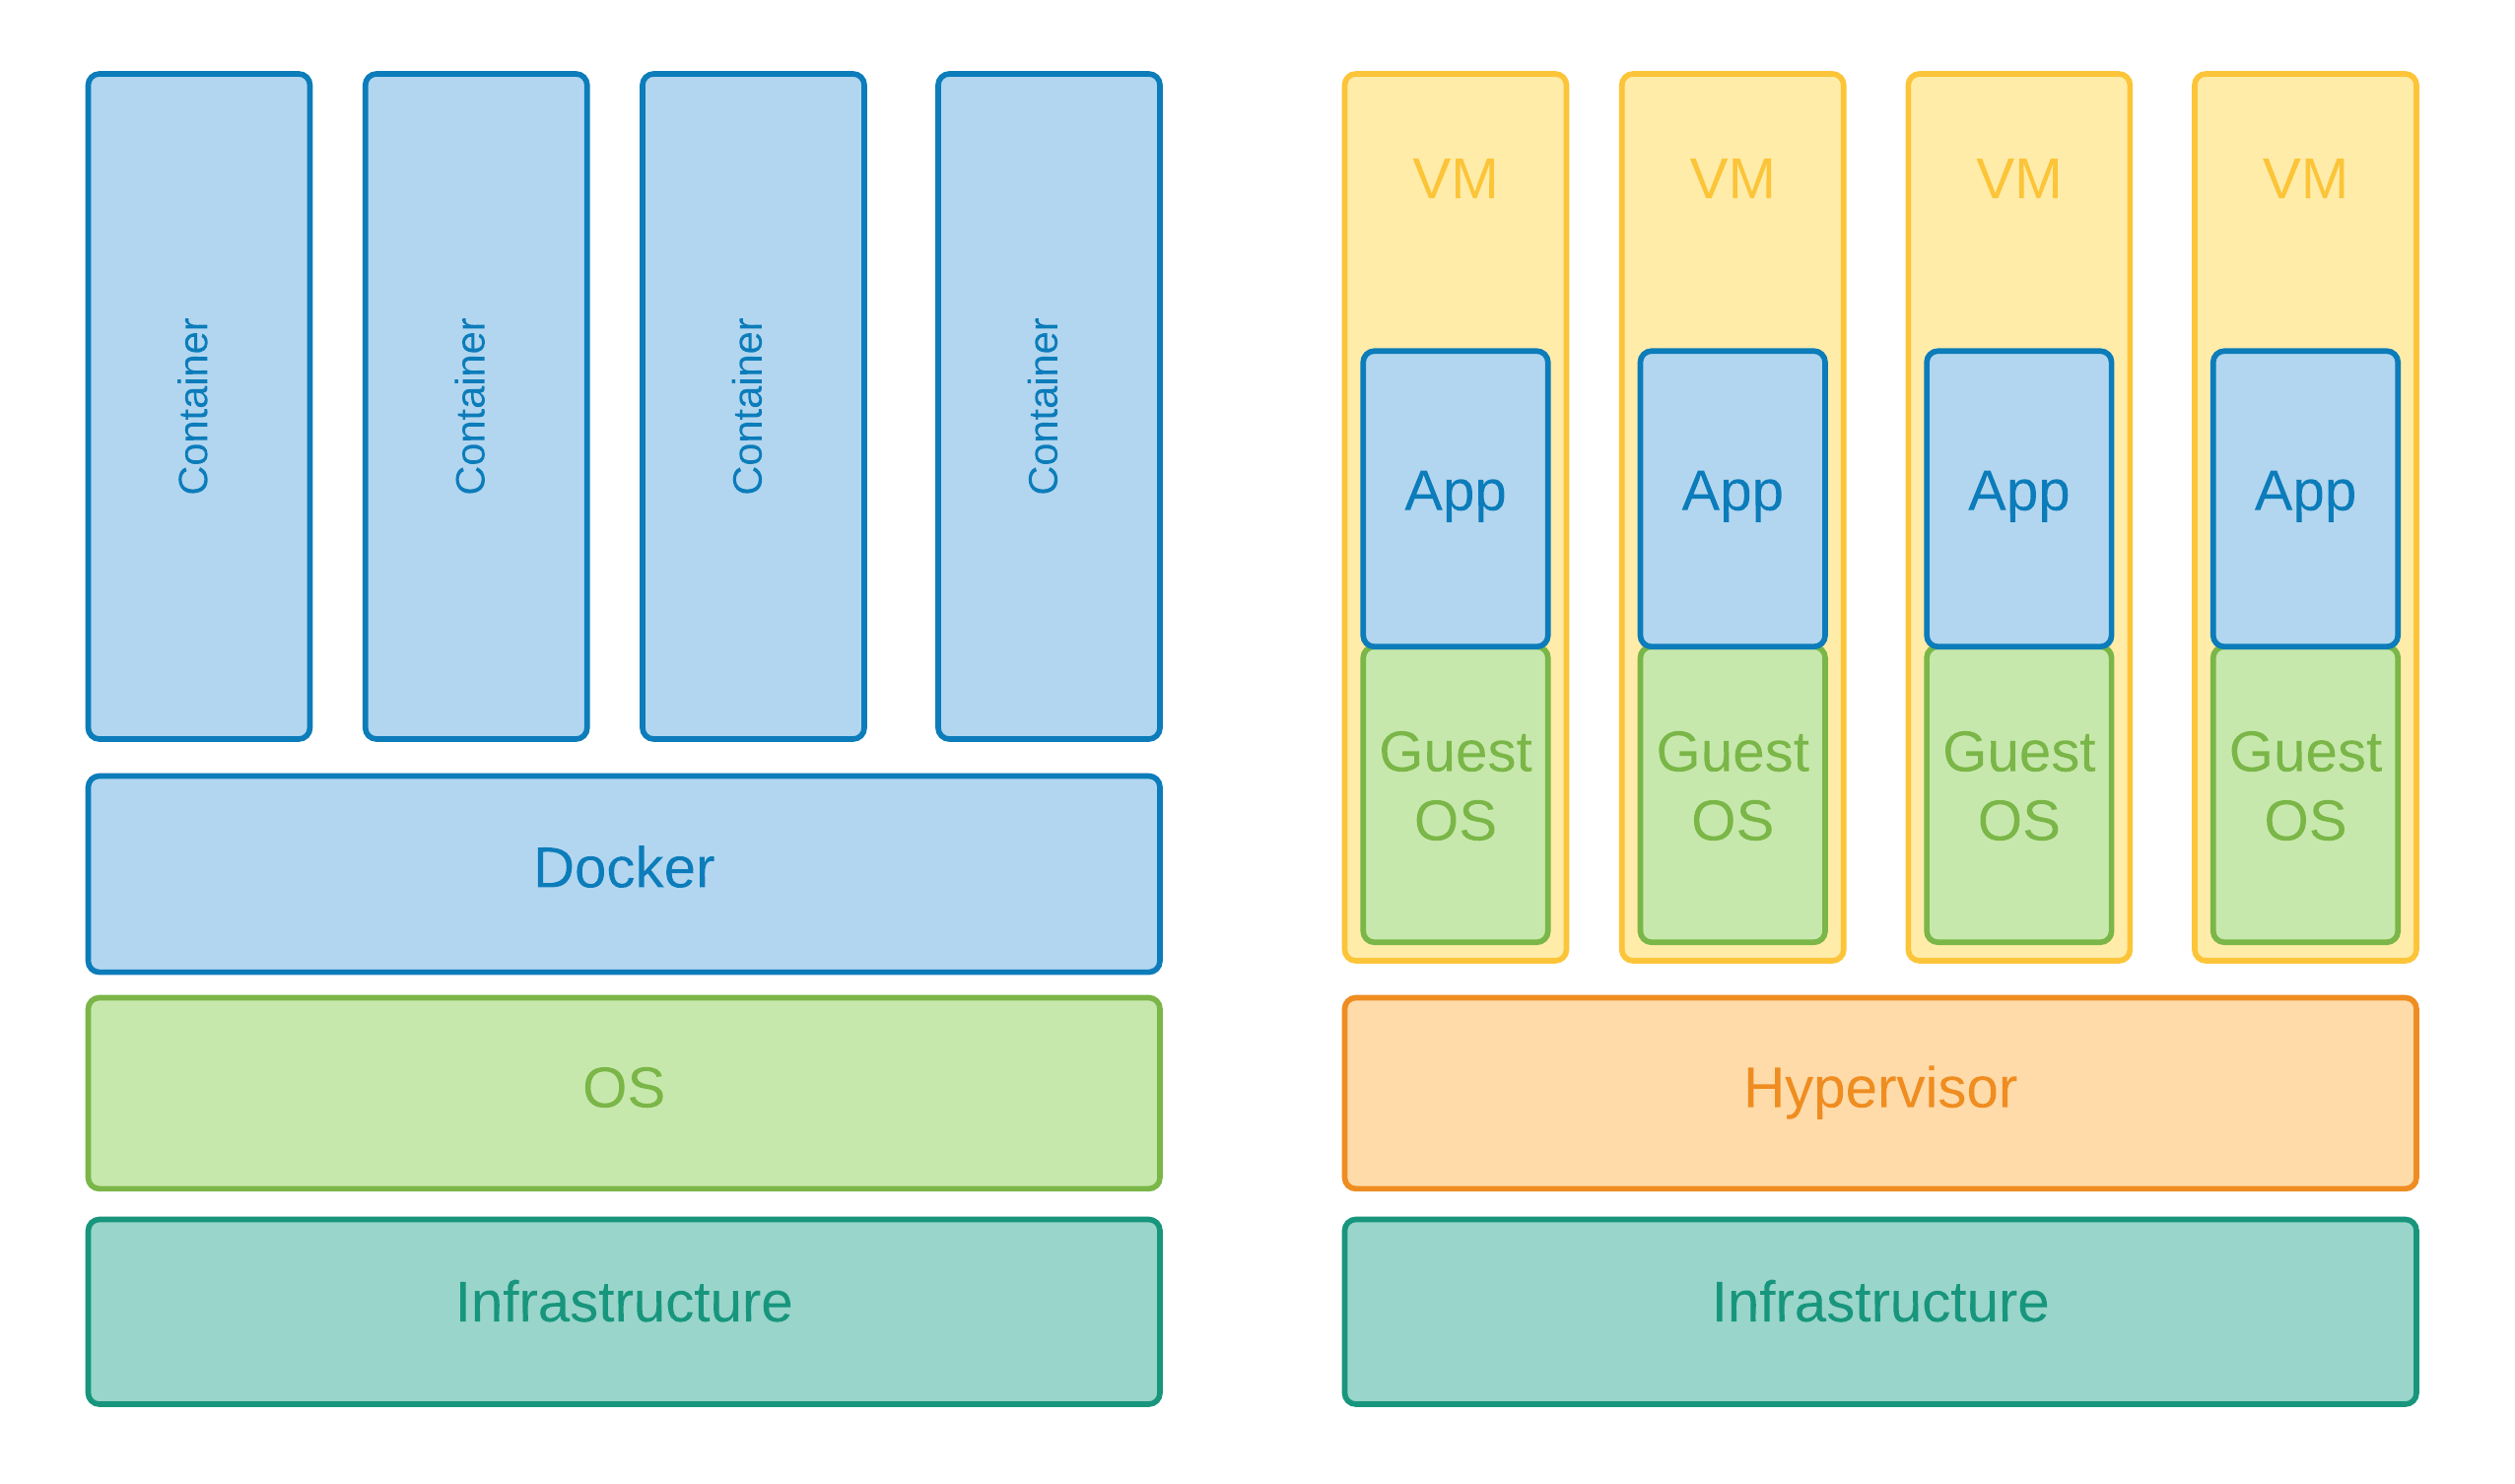
\includegraphics[width=1.0\columnwidth]{images/Container-VM.png}
    \caption{Virtualisierungsmöglichkeiten \protect}
    \label{fig:containervm}
\end{figure}

Die Einsparung von Ressourcen und dem einfachen bereitstellen auf Hostsysteme,
prädestinieren containerisierte Anwendungen für die Verwendung von Microservices
auf Container Plattformen wie Kubernetes.


\section{Kubernetes}

Dieser Abschnitt befasst sich zunächst mit den einzelnen Komponenten der Kubernetes Architektur.
Hinleitend werden spezielle Themen wie k3s, Hybrid Cloud und Rancher näher erläutert.
Kubernetes ermöglicht die Orchestrierung von containerisierten Arbeitslasten
und Services. Seit 2014 hat Google das Open-Source-Projekt zur Verfügung
gestellt und baut auf 15 Jahre Erfahrungen mit Produktions-Workloads \cite{kubernetes}.

\subsubsection{Namensgebung}
\glqq Der Name Kubernetes stammt aus dem Griechischen, bedeutet Steuermann oder Pilot, [...]
K8s ist eine Abkürzung, die durch Ersetzen der 8 Buchstaben \glqq ubernete\grqq{} mit \glqq 8\grqq{} abgeleitet wird\grqq{} \cite{kubernetes}.

\subsection{Cluster}
Die Zusammensetzung der beschriebenen Kubernetes Komponenten ergeben ein Kubernetes Cluster (vgl. Abbildung~\ref{fig:cluster}).


\begin{figure}
    \centering
    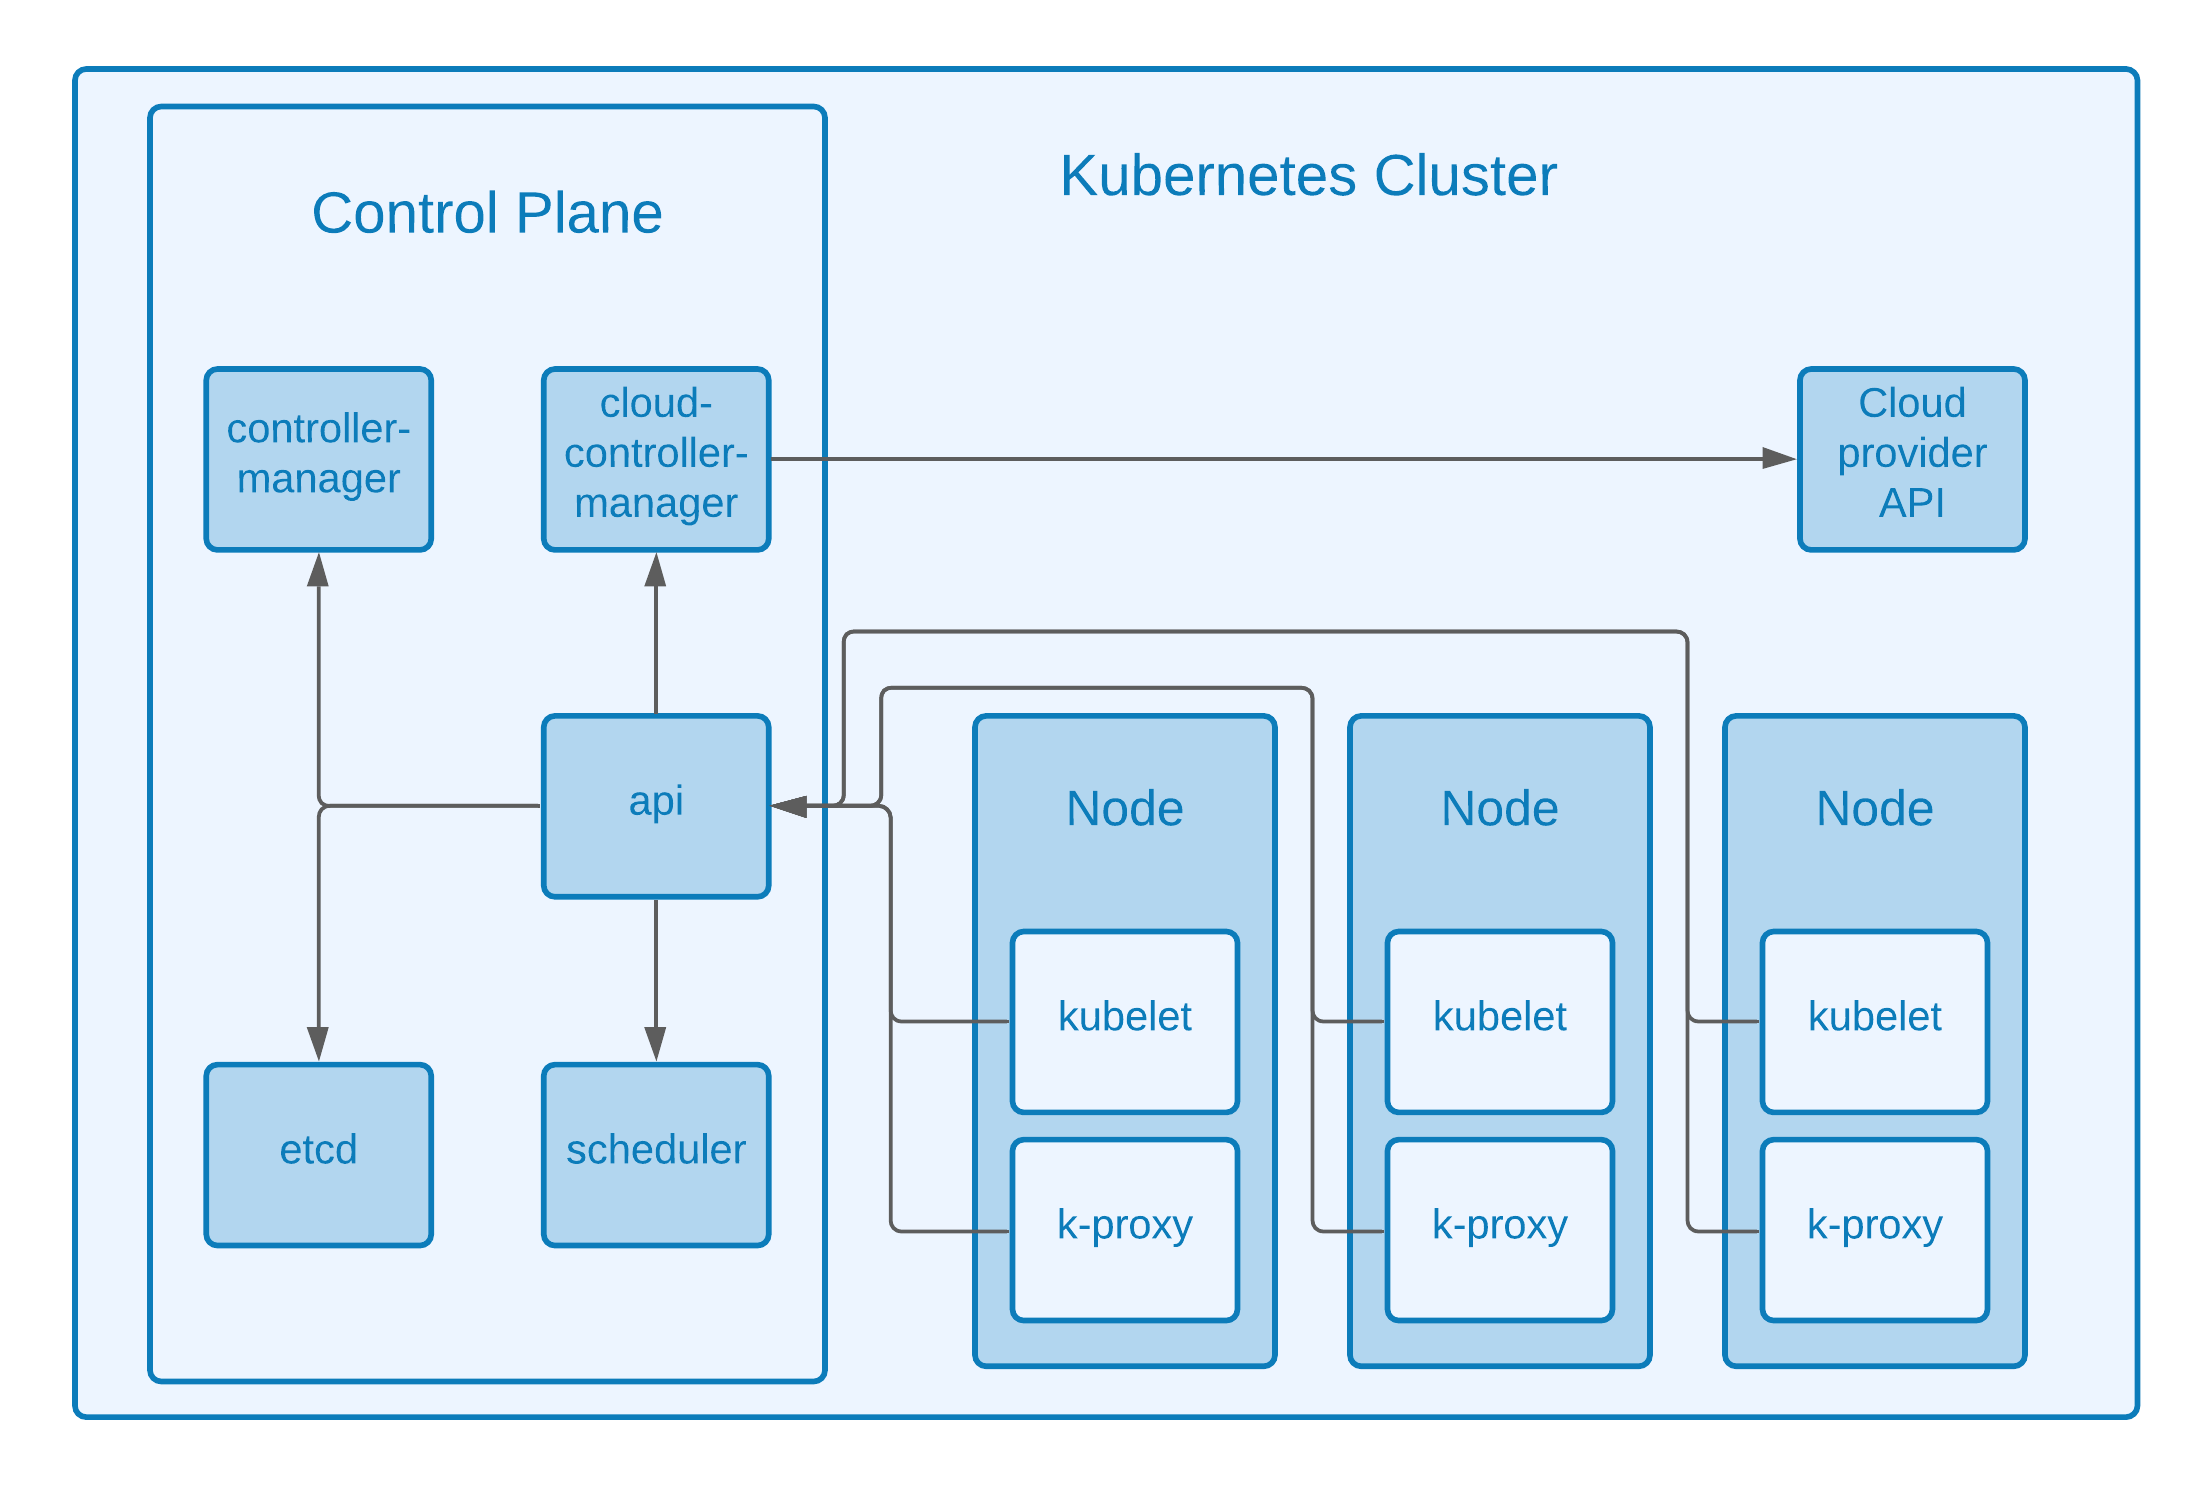
\includegraphics[width=1.0\columnwidth]{images/KubernetesKomponenten.png}
    \caption{Komponenten eines Kubernetes Cluster in Anlehnung an \cite{kubernetesnodekomponenten}.}
    \label{fig:cluster}
\end{figure}

\subsubsection{Control Plane}
Control Planes\footnote{Seit Kubernetes v1.20, ist die korrekte Bezeichnung für die Master Node Control Plane \cite{Kuberneteschangemaster}} sind für die Steuerungsebene des Clusters zuständig,
dabei entscheidet und reagiert dieser auf globaler Ebene auf eintreffende Clustereignisse \cite{kuberneteskomponenten}.
Die nächsten Unterabschnitte beschreiben diese näher:

\subsubsection{\textit{API Server}}
Der API Server operiert über REST und bietet eine Schnittstelle zu Diensten
inner- und außerhalb der Master-Komponenten \cite{kuberneteskomponenten}.

\subsubsection{\textit{etcd}}
etcd ist der primäre Datenspeicher von Kubernetes und sichert alle Zustände eines
Cluster \cite{kuberneteskomponenten}.

\subsubsection{\textit{Scheduler}}
Der Scheduler ist zuständig für die Verteilung und Ausführung von Pods auf Nodes \cite{kuberneteskomponenten}.

\subsubsection{\textit{Controller Manager}}
Der Controller Manager reagiert auf Ausfälle von Nodes, erhält die korrekte
Anzahl von Replikationen eines Pods und verbindet Services miteinander \cite{kuberneteskomponenten}.

\subsubsection{Node}
Eine Node\footnote{Um den Sprachfluss zu wahren wird der englische Begriff Node, als Kubernetes Ressourcenobjekt nicht übersetzt. 
Die Übersetzung Knoten findet als Hardwareinstanz statt.} 
ist eine Hardware Einheit, die je nach Kubernetes Einrichtung eineVM, physische Maschine oder 
eine Instanz in einer privaten oder öffentlichen Cloud darstellen kann \cite{kubernetesnodes}.
Dieser umfasst folgende Komponenten:

\subsubsection{\textit{Container Laufzeit}}
Der Abschnitt \hyperref[Docker]{2.1} beschreibt bereits alles zu diesem Thema.
Ergänzend dazu die Information, dass seit 2020 containerd als Auslaufmodell für die unterliegende Container Laufzeit, 
für die Kubernetes Versionen nach v1.20 auslaufen. Dies beeinträchtigt die spätere Implementierung dieser Arbeit aber nicht,
da k3s containerd als standard Laufzeit verwendet wird.

\subsubsection{\textit{Kubelet}}
Kubelet fungiert als \glqq node agent\grqq{} und registriert die Node mit dem
API-Server eines Clusters, dabei stellt es sicher das Container innerhalb eines Pods
funktionieren \cite{kubernetesnodes}.

\subsubsection{\textit{Kube-Proxy}}
Ein Kube-Proxy ist ein Netzwerk Proxy und verwaltet die Netzwerkrechte auf Nodes.
Diese erlauben die Kommunikation zwischen Pods inner- und außerhalb des Clusters \cite{kubernetesnodes}.

\subsection{Pods}
Ein Pod stellt die kleinste Einheit eines Kubernetes Clusters dar und ist eine Gruppe von mindestens einem Container.
Dieser erlaubt die gemeinsame Nutzung von Speicher- und Netzwerkressourcen mit Anweisungen zur Ausführung der Container \cite{kubernetespods}.

\subsection{Deployment}
Ein Deployment ist ein Ressourcenobjekt, dass mit einem Deployment Controller den gewünschten Zustand einer Anwendung aufrechterhält.
Diese Spezifikationen sind in Form von YAML-Dateien definiert (vgl. Beispiel~\ref{lst:deployment}).
Desweiteren eine kurze Aufschlüsselung der einzelnen Instruktionen \cite{kubernetesobjects}.
\begin{itemize}
    \item \textbf{apiVersion}: definiert die einzelnen workload API Untergruppen und die Version.
    \item \textbf{kind}: bestimmt das zu erstellende Kubernetes Objekt.
    \item \textbf{metadata}: deklariert einzigartige Bestimmungsmerkmale.
    \item \textbf{spec}: gewünschte Ausgangszustand des Objekts.
\end{itemize}

\begin{lstlisting}[caption={deployment.yaml \cite{kubernetesdeployment} },captionpos=b,label={lst:deployment},language=yaml]
    apiVersion: apps/v1
    kind: Deployment
    metadata:
      name: nginx-deployment
      labels:
        app: nginx
    spec:
      replicas: 3
      selector:
        matchLabels:
          app: nginx
        spec:
          containers:
          - name: nginx
            image: nginx:1.14.2
            ports:
            - containerPort: 80
    \end{lstlisting}

\subsubsection{Deployments und Pods}
Das Einbinden von Pods in Deployments ermöglicht Kubernetes das beziehen von 
wertvollen Metadaten für die Verwaltung von Skalierbarkeit,
Rollouts, Rollbacks und Selbstheilungsprozesse \cite{kubernetesnigeldeployments}. Der höhere Grad an Abstraktion
dient auch zur Aufteilung von Microservice Stacks, zum Beispiel dem aufteilen
von Frontend und Backend Pods in eigene Deployment Zyklen.

\subsection{Service}
Ein Service ist für die Zuweisung von Netzwerkdiensten einer logischen Gruppe Pods zuständig.
Services dienen als Abstraktion von Pods und ermöglichen die Replizierung und Entfernung
von Pods ohne Beeinträchtigung der laufenden Anwendung \cite{kubernetesservice}.

Pods beanspruchen Netzwerkressourcen, wie IP-Adresse und DNS-Name 
innerhalb ihres Clusters. Der Ausfall oder die Zerstörung eines Pods führt zu Beeinträchtigung der Kommunikation
zwischen Anwendungen. Services können dies präventiv verhindern, indem sie mit
selector und labeler eine Kommunikation zwischen zwei Kubernetes Objekten etablieren.
Das Beispiel zeigt eine solche Konfiguration (vgl. Beispiel~\ref{lst:service}). 
Die einzelnen Spezifikationen werden folgendermaßen definiert \cite{kubernetesservice}:

\begin{itemize}
  \item \textbf{selector}: definiert die Abbildung auf ein Label.
  \item \textbf{app}: führt den Service für Pods mit dem vorgegebenen Label aus.
  \item \textbf{ports}: Netzkonfiguration zwischen Service und Pod.
  \item \textbf{targetPort}: Port auf dem die Anwendung im Pod lauscht.
  \item \textbf{port}: Port auf dem der Service lauscht.
\end{itemize}

\begin{lstlisting}[caption={zum deutlicheren Verständnis mit dem deployment.yaml, leicht abgewandelte service.yaml \cite{kubernetesservice} },captionpos=b,label={lst:service},language=yaml]
    apiVersion: v1
    kind: Service
    metadata:
      name: my-service
    spec:
      selector:
        app: nginx
      ports:
        - protocol: TCP
          port: 80
          targetPort: 9376
    \end{lstlisting}

Bei der Erstellung eines Services wird ein REST Objekt erstellt, dass mithilfe eines Controller kontinuierlich 
nach Pods mit dem passenden Selector sucht, welcher jegliche Updates als POST-Anfragen schickt.


\subsection{Ingress}

Ein Ingress ist ein Kubernetes Ressourcenobjekt, dass die Verfügbarkeit von internen Services auf öffentliche Endpunkte ermöglicht.
Diese Routen werden mittels HTTP oder HTTPS freigegeben und können in Form einer URL verwendet werden \cite{kubernetesingress}.
Die Anforderung für die Implementierung eines Ingress ist der Ingress-Controller, eine Vielzahl an Optionen dafür wird in der 
Dokumentation aufgelistet \cite{kubernetesingresscontroller}. Für die Realisierung des Prototyps kommt ein NGINX Ingress Controller in Einsatz, weshalb
dieser näher erläutert wird.

\subsubsection{NGINX Ingress Controller}
Der Ingress Controller ist für die Umsetzung einer vorgegebenen Objektspezifikation zuständig \cite{kubernetesingress}.
Die übliche Verwendung eines Controllers beeinhaltet die Lastenverteilung durch weiterleiten des Datenverkehrs an Services. 
Diese Kommunikation findet, wie auch bei dem NGINX Ingress Controller \cite{kubernetesingresscontrollerlayer} in der Anwendungsschicht des OSI-Schichtenmodells statt und ermöglicht, dadurch die 
Lastenverteilung von öffentlichen Endpunkten zu internen Pods in einem Cluster \cite{kubernetesingressibm}.
Wie in alle anderen Kubernetes Objekten auch werden vordefinierte Aufgaben des Ingress Controller durch YAML-Dateien abgebildet (vgl. Beispiel~\ref{lst:ingress}).
Im folgenden wichtige Optionen die etwas genauer erklärt werden:

\begin{itemize}
  \item \textbf{ingressClassName}: definiert den Ingress Controller.
  \item \textbf{rules}: die Zusammsetzung der einzelnen HTTP Regeln.
  \item \textbf{host}: definiert das Ziel des eintreffenden Datenverkehrs.
  \item \textbf{paths}: gibt die Endpunkte des verbundenen Service an.
  \item \textbf{backend}: leitet die Anfragen an den Service mit der richtigen Port Zuweisung weiter.
\end{itemize}

\begin{lstlisting}[caption={ingress.yaml \cite{kubernetesingress} },captionpos=b,label={lst:ingress},language=yaml]
  apiVersion: networking.k8s.io/v1
  kind: Ingress
  metadata:
    name: minimal-ingress
    annotations:
      nginx.ingress.kubernetes.io/rewrite-target: /
  spec:
    ingressClassName: nginx
    rules:
    - http:
        paths:
        - path: /testpath
          pathType: Prefix
          backend:
            service:
              name: test
              port:
                number: 80
  \end{lstlisting}

\subsection{Lightweight Kubernetes} \label{k3s}
Ligthweight Kubernetes auch K3s genannt ist eine Open-Source Kubernetes Distribution von dem Unternehmen
Rancher. Der größte Unterschied der Distribution ist die einnehmende größe 
auf Hostsystemen mit einer einzelnen Binärdatei von nur 40MB ist auch Platz auf kleineren Geräten.
Durch die Verschlankung der Distribution ist der ideale Anwendungszweck für IoT oder Edge-Devices mit wenig Rechenleistung.
Denn die minimalen Systemanforderungen für Hostsysteme liegen bei einem 512MB-RAM Speicher und einer Pi4B BCM2711, 1.50 GHz CPU\footnote{Einplatinencomputer Raspberry Pi 4B, basierend auf ARM \cite{pi4} } \cite{k3sAnforderung}.
Der hauptsächliche Verwendungszweck von k3s liegt in IoT und Edge-Devices, da unwichtige Kubernetes Inhalte entfernt wurden. \cite{k3s}.
Trotz dieser Reduzierung, bleiben die Kernfunktionalitäten von Kubernetes erhalten und werden 
so weit wie möglich parallel auf dem neusten Stand gehalten \cite{k3sgit}.

\begin{figure}
  \centering
  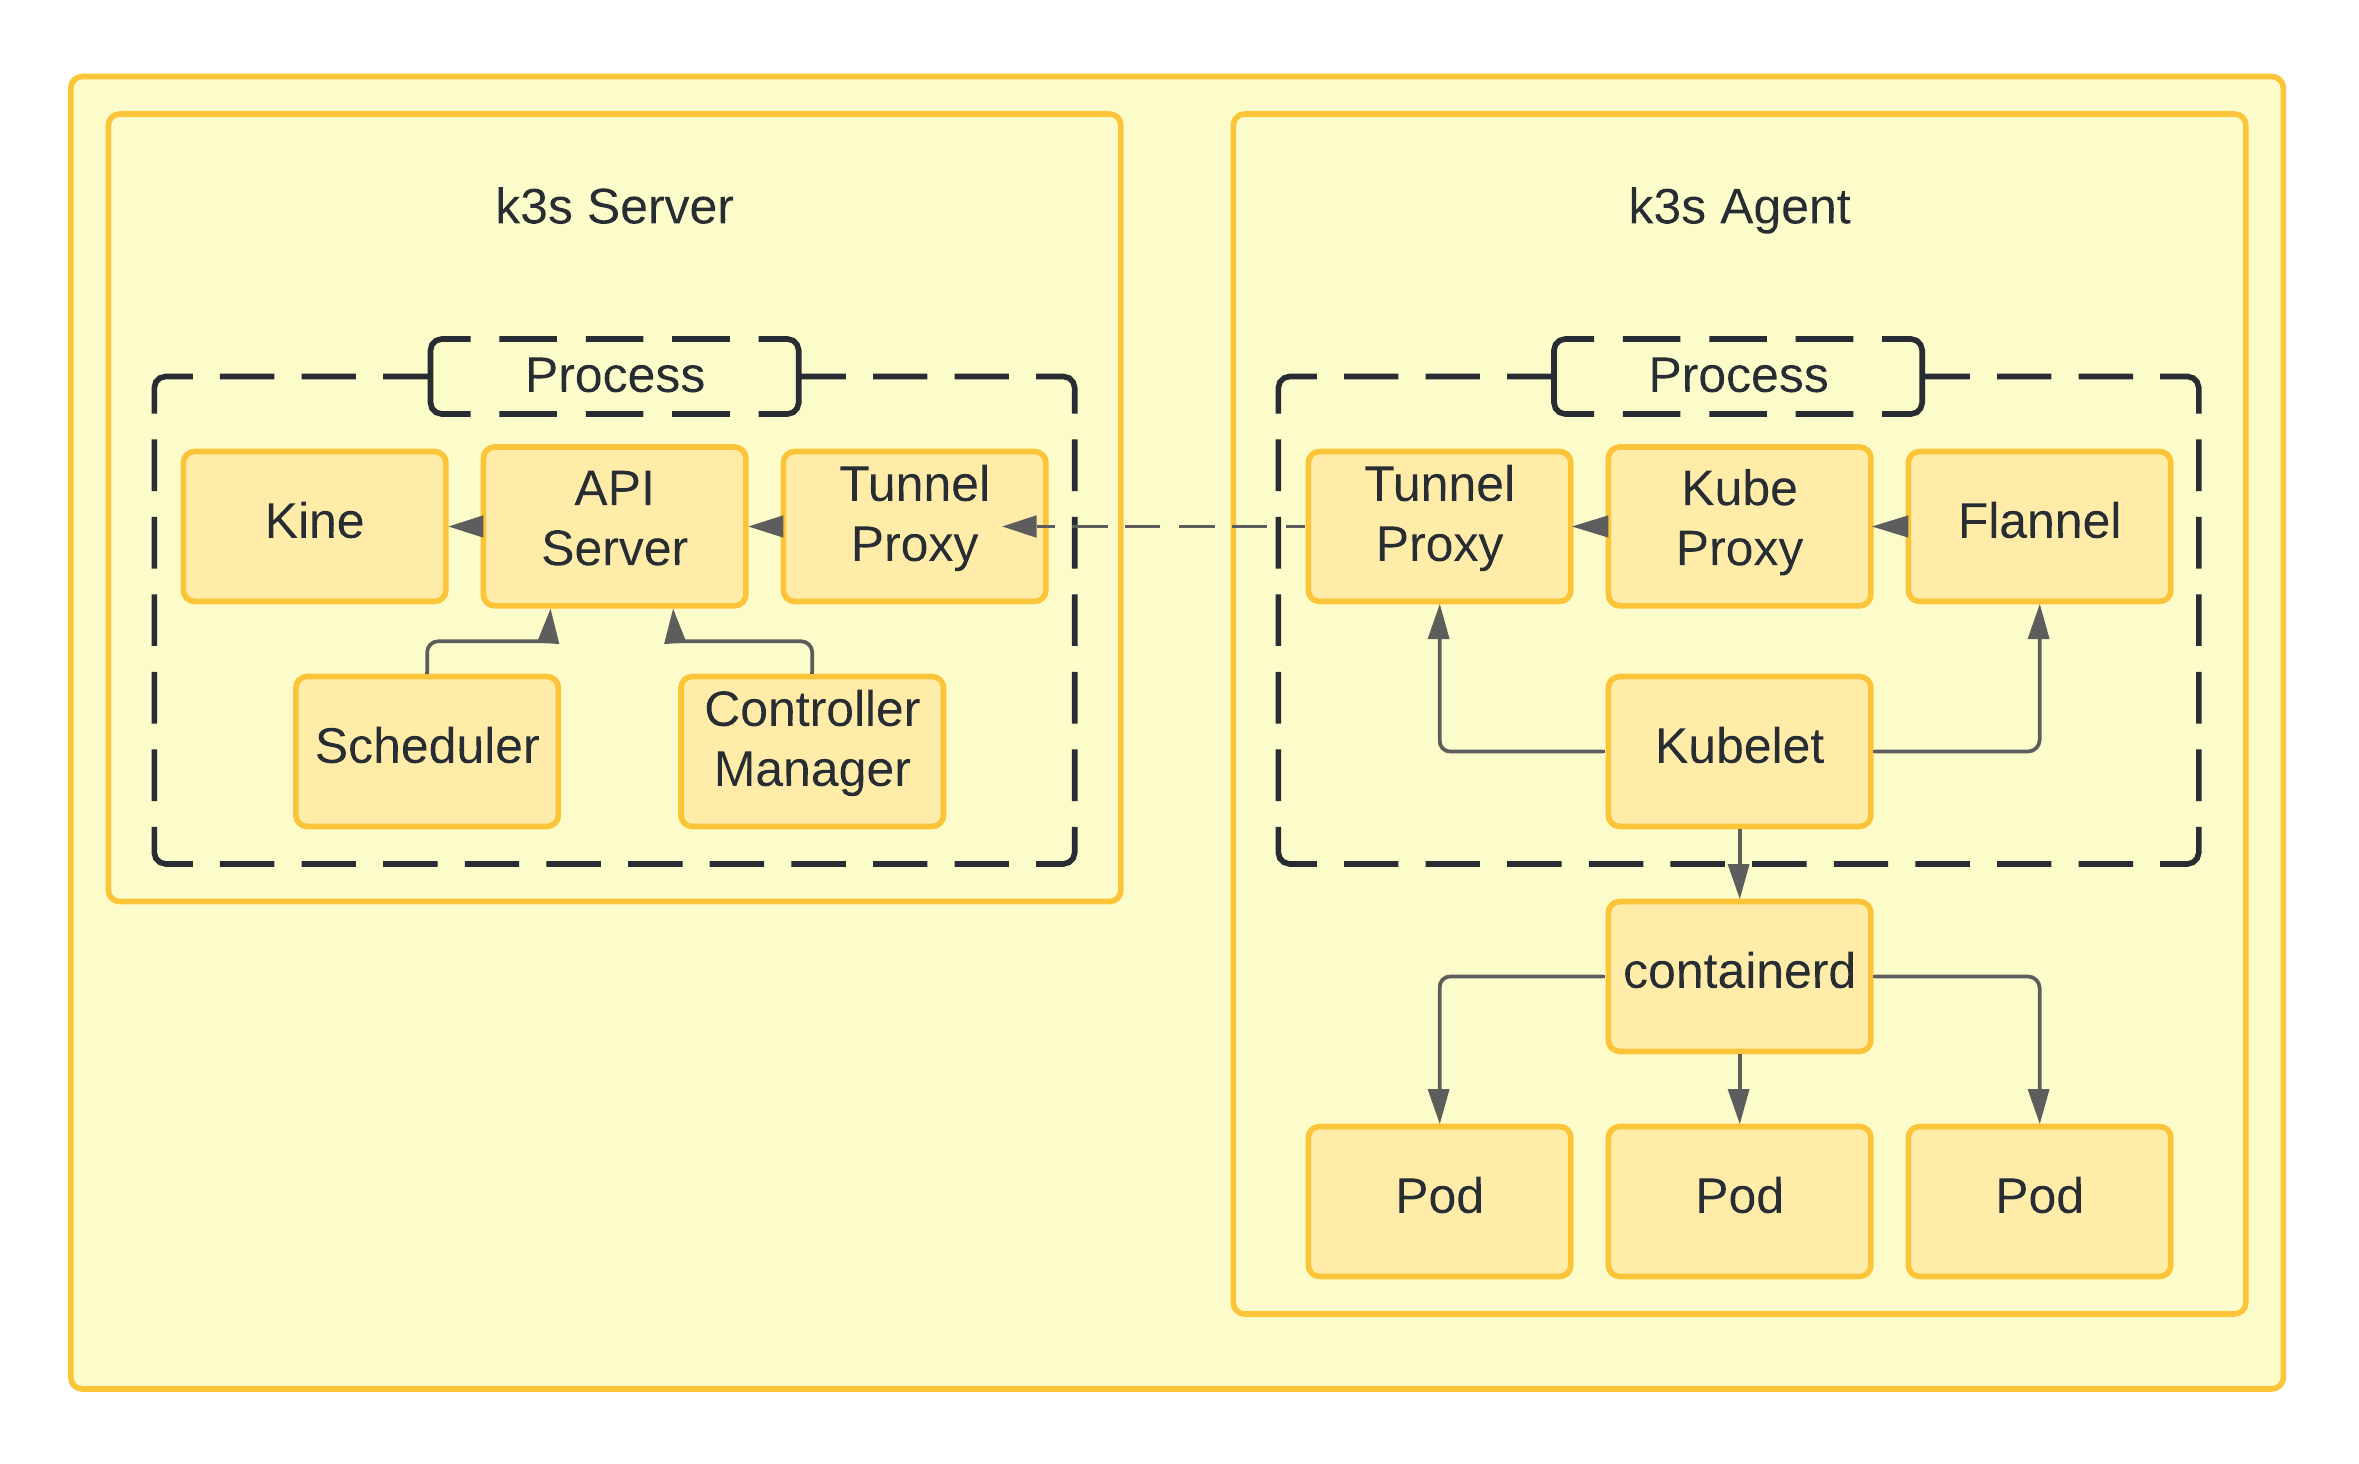
\includegraphics[width=1.0\columnwidth]{images/K3sArchitektur.png}
  \caption{K3s Architektur in Anlehnung an \cite{k3sarch}.}
  \label{fig:k3sarchitektur}
\end{figure}

\subsubsection{Besonderheiten}
Die Abbildung \ref{fig:k3sarchitektur} zeigt die Architektur von k3s auf. Das Kubernetes äquivalent zur Control Plane und Node
sind Server und Agent. Eine Besonderheit dessen ist, das Server parallel einen Agent Prozess auf dem selben Knoten starten und
somit Arbeitslasten mithilfe von Kubelet ausführen \cite{k3sServerAgent}. Weiterhin wird im Gegensatz zu Kubernetes containerd weiterhin unterstüzt und
kommt vorinstalliert mit Kubelet \cite{k3s}. Zwei weitere Unterschiede werden näher erläutert:

\textbf{Kine}
das Akronym steht für 'Kine is not etcd' und ist eine Abstraktionsschicht für etcd, welche sqlite, Postgress, Mysql und dqlite übersetzt \cite{k3sgit}.
Dadurch kann der Backend Speicher des Clusters durch die oben genannten Datenbanksysteme ersetzt werden.

\textbf{Flannel}
ist ein überlagerndes Netzwerkmodell in k3s und ermöglicht IPv4 Netzwerke innerhalb eines Clusters mit mehreren Knoten.
Dazu wird eine einzelne Binärdatei gestartet, welche Agents auf Hostssystemen startet und alloziert Subnetze in einem vorkonfigurierten Adressraum.
Das Modell ist dabei für die Übertragungsart des Datenverkehrs zwischen unterschiedlichen Knotenpunkten zuständig.
Die Speicherung der Netzwerkkonfiguration erfolgt über etcd oder der Kubernetes API \cite{flannel}.


\subsection{Rancher}
In diesem Unterabschnitt wird die Open-Source Lösung Rancher von dem gleichnamigen Unternehmen zur Orchestierungs von Kubernetes Clustern näher behandelt.
Diese ermöglicht, das Verwalten von Kubernetes Clustern auf der eigenen Infrastruktur, sowohl vor Ort als auch in der Cloud.
Die Bereitstellung von Clustern mittels Rancher ist Cloud-Anbieter unabhängig,
weshalb Cluster in der Praxis mit der selben Rancher Instanz auf AWS, Azure oder anderen Cloud-Anbietern betreut werden können \cite{rancher}.

Die Rancher Benutzeroberfläche vereinfacht das steuern von Arbeitslasten, auf einer zentralen administrativen Instanz, welche gleichzeitig Authentifizierung und Rechteverteilung von Benutzern anbietet.
Das grundsätzliche verwalten von Arbeitslasten verlangt kein tiefgründiges Wissen bezüglich Kubernetes Konzepte. 
Die mitgelieferten Tools ermöglichen die Auslieferung und Verbindung von Kubernetes Objekten und abstrahieren die Komplexität, die für die Betreuung eines solchen Systems notwendig sind \cite{rancher,AzureKubernetesService}.

Für komplexere Konfigurationen, kann über die Oberfläche ein Terminal mit Kubectl aufgerufen werden.
Wie auch in Kubernetes ist der Zugang auf ein Kubernetes Cluster von einer lokalen Entwicklungsumgebung mit einer kubeconfig-Datei möglich, diese beeinhaltet die Adresse zum Rancher Server, Nutzerrechte und Zertifizierungszeichen \cite{rancherKubeconfig}.

\begin{figure}[!htb]
  \centering
  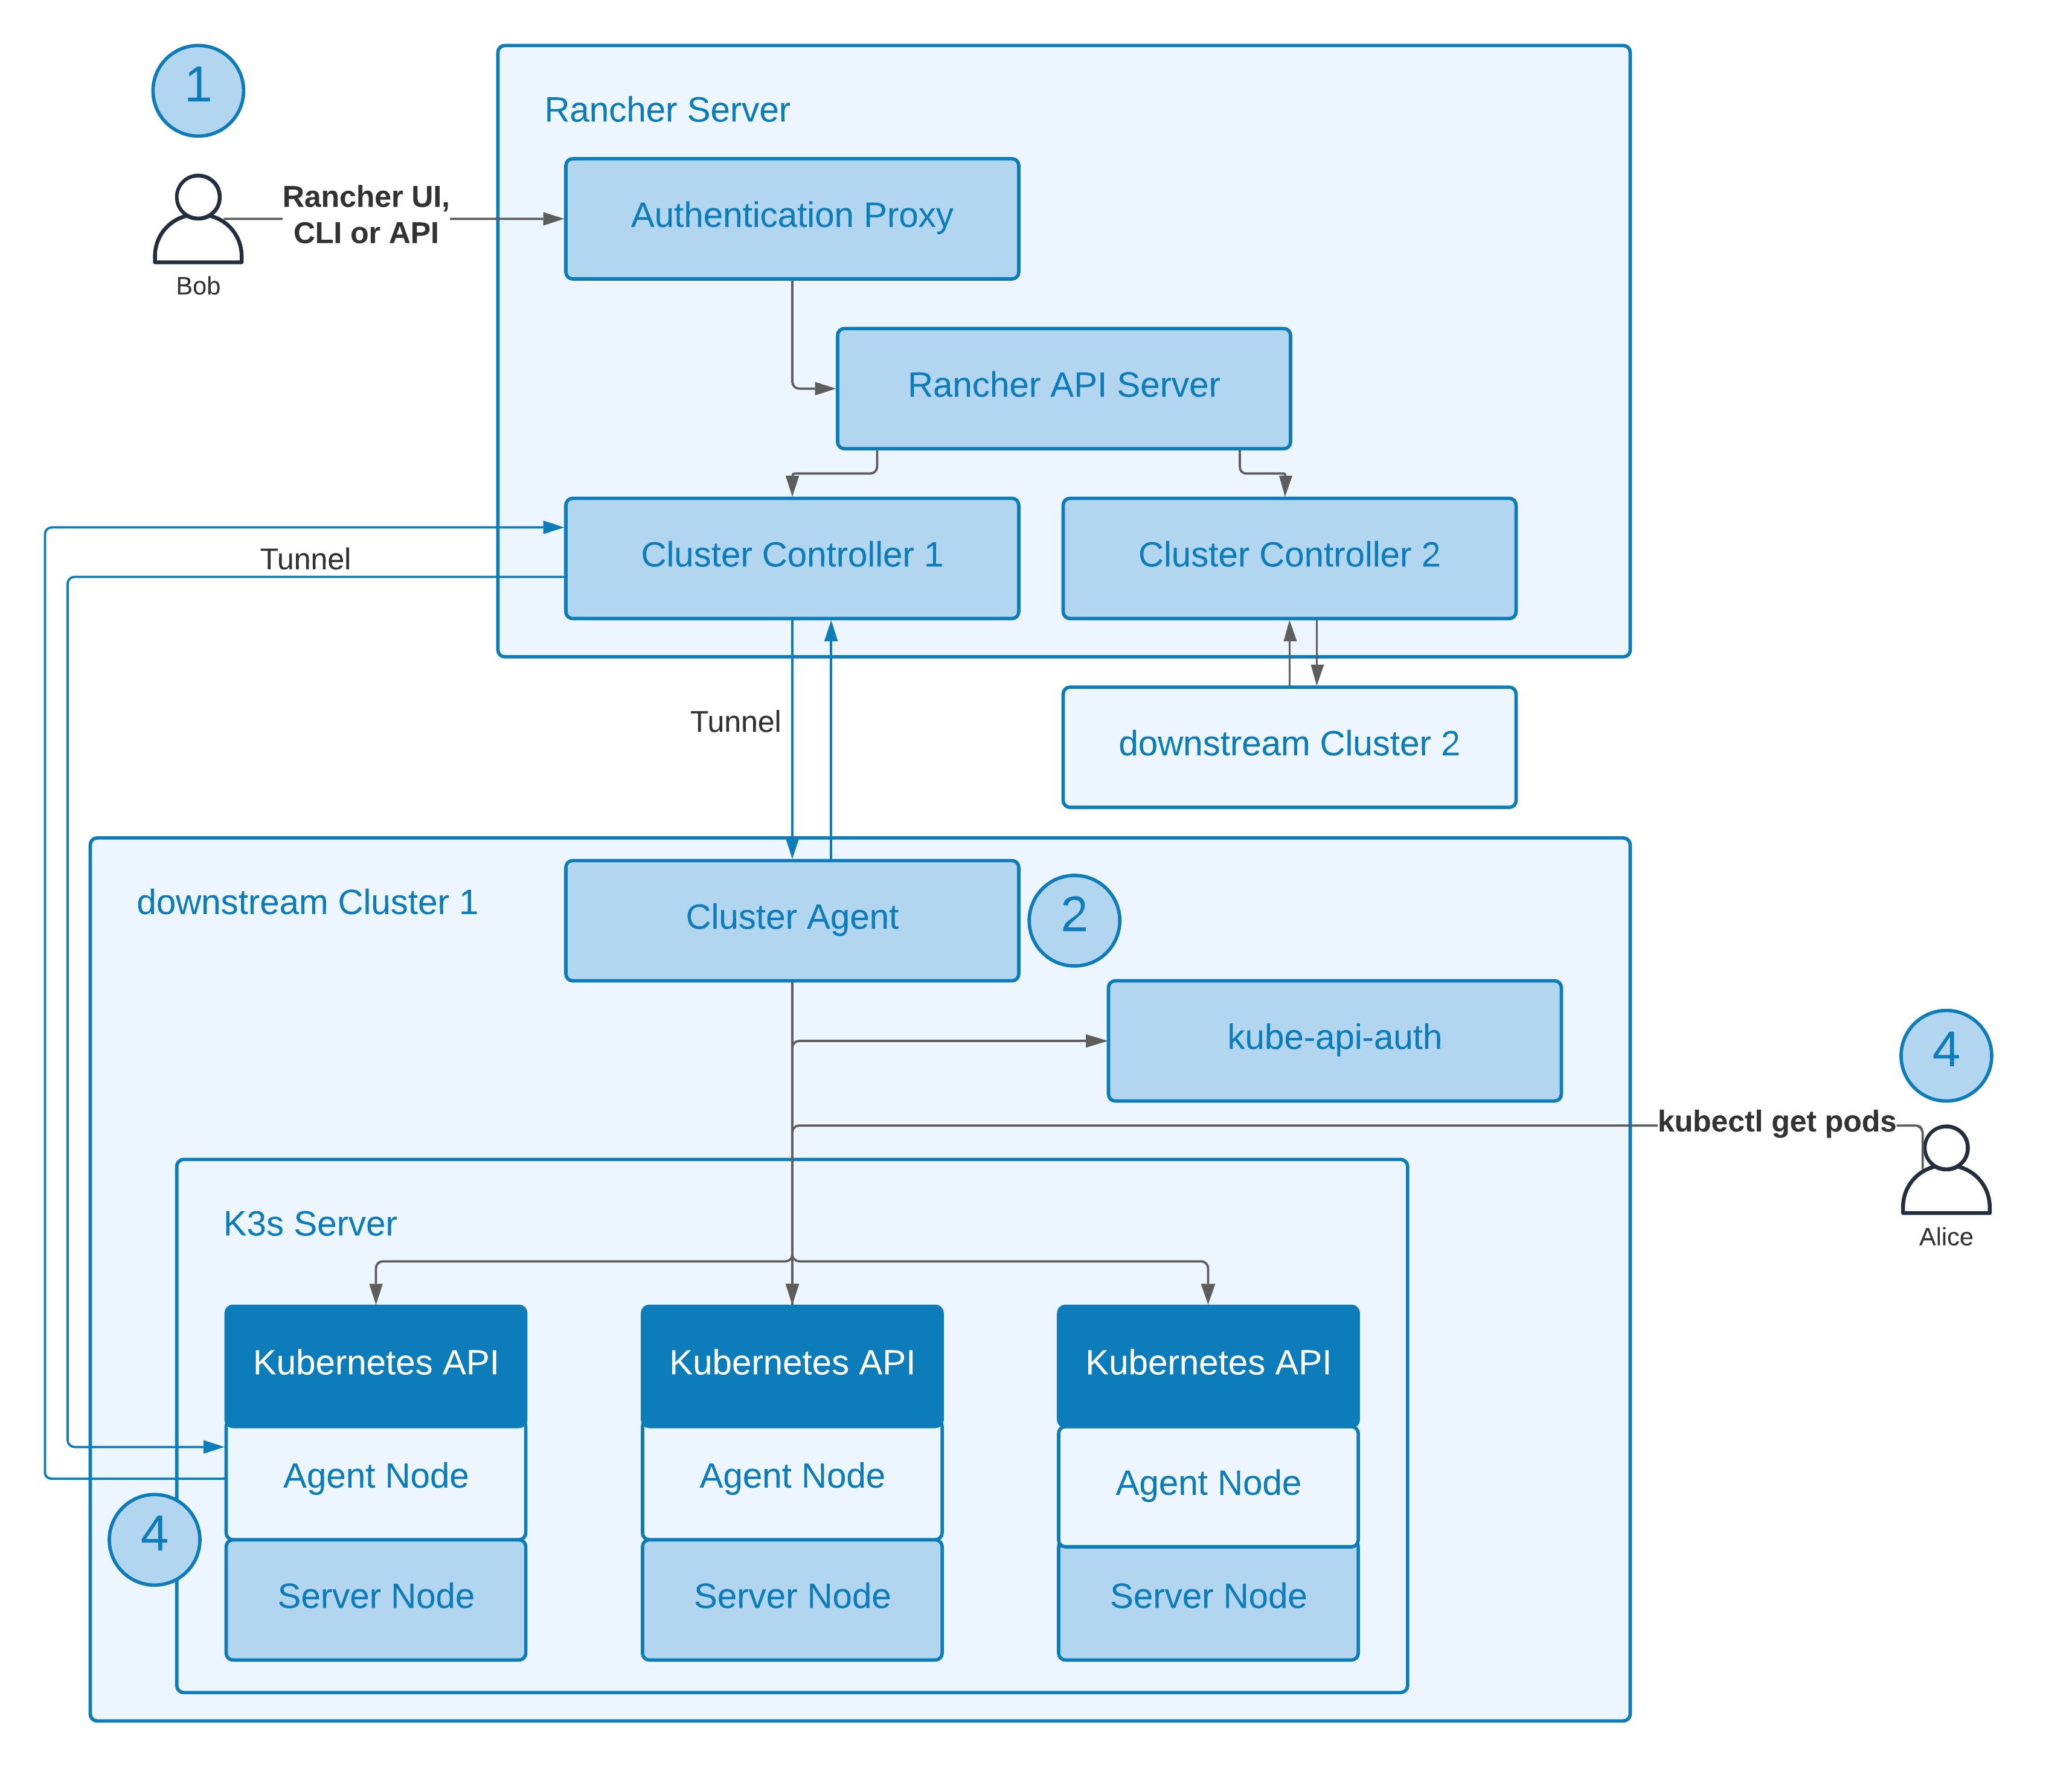
\includegraphics[width=0.8\columnwidth]{images/RancherArchitekturClusterController.png}
  \caption{Rancher Server Kommunikation mit einem downstream k3s Cluster, überarbeitete Abbildung von \cite{rancherArchitecture}. (Im Sinne der späteren Architektur nachgebildet)}
  \label{fig:rancherarchitektur}
\end{figure}

Die Abbildung \ref{fig:rancherarchitektur} zeigt den Vorgang von Zwei Benutzern, 
die auf ein von Rancher verwalteten downstream k3s Cluster\footnote{Die offiziele Bezeichnung für ein Kubernetes Cluster unter Rancher ist \textbf{downstream Cluster} \cite{rancherArchitectureRecommendations}} zugreifen.
Die nachfolgende Beschreibung aus der Dokumentation gibt die einzelnen Schritte mit der in der Abbildung nummerierten Posten wieder \cite{rancherArchitecture}.


\begin{enumerate}
\item Zuerst authentifiziert sich Bob mit seinen Benutzerdaten bei dem Authentifizierungs-Proxy an seinem Rancher Server.
Dieser Proxy leitet den Aufruf, über eine Kommandozeile oder der Rancher Benutzeroberfläche mit der ausgewählten downstream-Cluster Instanz weiter und führt diese aus.
Dafür wird vor dem weiterleiten des Aufrufs, der angemessene Kubernetes Impersonation Header gesetzt, 
welcher sich als Service Account der Rancher Instanz ausgibt und je nach Benutzerstatus reagiert.   
\item Die Übertragung des Aufrufs erfolgt über einen Cluster-Controller auf dem Rancher Server
und dem parallel laufendem Cluster-Agent des downstream-Cluster. Der Controller ist für die Überwachung, Veränderung
und Konfiguration von Zuständen auf dem laufendem Cluster zuständig. 
\item Wenn der Cluster-Agent nicht erreichbar ist,
werden die Aufrufe an den Node-Agent\footnote{Ein Rancher DaemonSet zur Interaktion mit Nodes, 
nicht zu verwechseln mit dem Node-Agent von k3s \cite{rancherAgents}. } überreicht, welcher standardmäßig auf jedem downstream-Cluster läuft.
\item Zuletzt hat auch die Benutzerin Alice, die Möglichkeit sich über einen autorisierten Cluster Endpunkt zu verbinden.
Denn jeder downstream-Cluster verfügt, über eine Kubeconfig, welche den Zugang ohne Authentifizierungs-Proxy erlaubt.
Durch den Microservice kube-api-auth wird eine Kommunikation, über einen Web-Haken realisiert, der die Verbindung
zwischen Alice Rechner aufbaut. 
Dies ermöglicht die Verwendung von Befehlszeilentools, wie Kubectl und Helm.
\end{enumerate}

%\section{Distributed Clouds}
%\subsection{Edge Computing}
\subsection{Hybrid Cloud}
Eine Hybrid-Cloud ist eine Kombination aus Öffentlichen-Cloud-Diensten und Privaten-Cloud-Diensten, die auf einer einzigen Infrastruktur laufen.
Dies ermöglicht die flexible Orchestrierung von Anwendungen, auf Hostssystemen vor Ort oder in der Cloud \cite{ibmHybrid}.

Der Schwerpunkt solcher Hybrid-Clouds liegt, dabei bei der Portierbarkeit der Arbeitslasten auf allen Cloud-Umgebungen.
Dafür ist die Aufbereitung oder Entwicklung, alter oder neuer Anwendungen für cloudnative Technologien nötig, mehr dazu im Abschnitt \ref{Microservice} zu Microservices.
Private-Clouds können auch von Drittanbietern, durch externe Rechnzentren, als Enterprise Modell angeboten werden, die Entwicklern eine Landschaft bietet
Hardware flexibel zu verändern. Dabei ist die Nutzung eines einzigen Betriebssystems ratsam, um Abhängigkeiten bei der Automatisierung von cloudnativen Anwendungen zu verhindern.
Die Verwaltung erfolgt, dabei mit einer Container-Orchestierungsplattform, wie Kubernetes und ermöglicht die nahtlose Implementierung von Cloud-Umgebungen \cite{ibmHybrid}.

\section{Microservice}\label{Microservice}
Microservices sind unabhängige Dienste, die mit anderen Diensten über ein Netzwerk kommunizieren \cite{BuildingMicroservicesNewman}.
Der folgende Abschnitt behandelt, zunächst die Architektur und dessen grunglegenden Aufbau.
Danach werden Schlüsselkonzepte behandelt und anschließend die Vor- und Nachteile der konkurrierenden monolitschen Architektur zusammengefasst.


\subsection{Architektur}
Der von Fowler häufig zitierte Artikel beschreibt den Microservice-Stil, als einen Ansatz für die Entwicklung einer einzelnen Anwendung, die wiederum aus vielen kleineren Diensten besteht.
Die jeweils mit eigenen Prozessen, miteinander über einfache Kommunikationsprotokolle wie HTTP kommunizieren.



\subsection{Konzepte}
\subsection{Vorteile}


%\subsubsection{Ein Unterabschnitt}
